\newpage
\setcounter{section}{0}
\renewcommand{\thesection}{\arabic{section}}

\begin{center}
    \Huge
    \textbf{Modul 3}
    
    Mengelola dan Membagi Bandwidth dengan Menggunakan QoS(Simple Queue) 

\end{center}


\section{pendahuluan}

Dalam lingkungan jaringan yang padat, sering kali beberapa pengguna menggunakan aplikasi atau protokol yang mengkonsumsi bandwidth yang tinggi, seperti video streaming atau file sharing, sementara pengguna lainnya mungkin hanya perlu menggunakan aplikasi yang membutuhkan bandwidth yang lebih rendah, seperti browsing web atau email. Tanpa manajemen bandwidth yang efektif, pengguna dengan aplikasi berat bisa mendominasi sebagian besar bandwidth, menyebabkan kualitas layanan yang buruk bagi pengguna lain.

\section{Tujuan Praktikum}

Mengetahui cara melimitasi dan memanagemen bandwidth untuk suatu jaringan dengan banyak pengguna.

\section{Alat dan Bahan}

Berikut adalah Alat dan Bahan untuk praktikum:
\begin{enumerate}
    \item 1 RouterOS Mikrotik
    \item 2 Laptop
    \item Kabel LAN 
    \item Software WinBox
\end{enumerate}

\section{Topologi}

berikut adalah topologi yang digunakan :

\begin{center}
    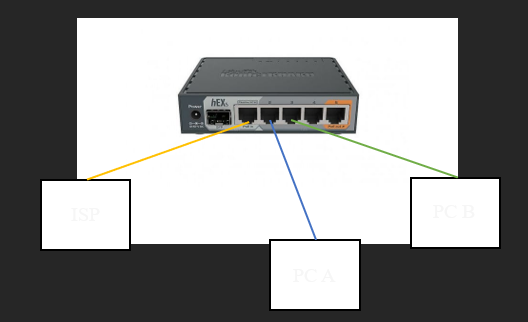
\includegraphics[width=0.7\textwidth]{image/P3/Topologi.png}    
    
    figure.1 Topologi
\end{center}


\section{Langkah Percobaan}
\begin{enumerate}
    \item Sambungkan PC dan router mikrotik sesuai dengan topologi
    \item Matikan firewall di laptop
    \item Masuk ke aplikasi Winbox
    \item Pada bagian Neighbour, check apakah ada IP 0000 identity mikrotik
    \item Reset mikrotik ke 0000
    \item Lalu tekan connect
    \item Lakukan konfigurasi DHCP agar dapat terhubung dengan ISP, pilih menu IP \texttt{\text>} DHCP Client \texttt{\text>} (+) \texttt{\text>} Interface : ether 1 (yang terhubung pada ISP)
    \item Kemudian secara otomatis akan didapatkan IP dari ISP
    \item Lalu pilih menu IP \texttt{\text>} Firewall \texttt{\text>} NAT \texttt{\text>} Chain : srcnat, Out. Interface : ether 1
    \item Kemudian pilih menu IP \texttt{\text>} Firewall \texttt{\text>} NAT \texttt{\text>} Action : masquerade
    \item Setelah itu atur routes untuk ether 1 secara static, pilih menu IP \texttt{\text>} Routes \texttt{\text>} (+) \texttt{\text>} Dst Address : 0.0.0.0/0, Gateway : (gateway IP address yang telah diberikan ISP) \texttt{\text>} Apply
    \item Setelah terlihat status “reachable” pada Route List, kemudian atur DNS
    \item Untuk melakukan limitasi bandwidth sederhana, pilih New Simple Queue \texttt{\text>} General
    \item Pada kolom Target Address, masukkan IP address yang akan diberikan limitasi
    \item Dan pada kolom Max Limit, masukkan besar maximum limitasi yang akan diberikan
    
\end{enumerate}

\section{Hasil Percobaan}


\section{Kesimpulan}

Pembatasan bandwidth suatu jaringan dapat dilakukan dengan menggunakan QoS(Simple Queue)

\section{Tugas modul}

\begin{enumerate}
    \item Manfaat dari implementasi QoS dalam manajemen bandwidth yaitu dapat memberikan prioritas layanan, pengendalian trafik, mengurangi latency,\\ meningkatkan kinerja aplikasi, dan mengoptimalkan penggunaan sumber daya.

    \item Situasi dimana prioritas bandwidth menjadi kritis yaitu dalam jaringan yang digunakan oleh beberapa penyewa atau pelanggan. QoS menjadi penting untuk memastikan pengalaman yang adil dan memenuhi kebutuhan masing-masing penyewa. Tanpa QoS, satu penyewa yang menggunakan sebagian besar bandwidth dapat mengorbankan kinerja dan kualitas layanan untuk penyewa lainnya. Dengan menerapkan QoS, prioritas bandwidth dapat diberikan berdas\\arkan kebutuhan dan kesepakatan kontrak dengan setiap penyewa, sehingga memastikan distribusi yang adil dan memenuhi persyaratan layanan.
    
    \item Risiko atau masalah yang mungkin muncul saat mengimplementasikan QoS salah satunya yaitu Konfigurasi QoS dapat menjadi kompleks, terutama dalam jaringan yang kompleks atau besar. Mengidentifikasi aplikasi atau layanan yang memerlukan prioritas bandwidth tertentu, mengatur aturan prioritas, dan mengelola kebijakan QoS dapat melibatkan pengaturan yang rumit. Kesalahan konfigurasi dapat mengakibatkan gangguan jaringan atau distribusi bandwidth yang tidak diinginkan.
    
    \item Perbedaan antara menggunakan QoS dengan Simple Queue dan menggunakan pembatasan bandwidth biasa, seperti limitasi bandwidth pada router, terletak pada tingkat kontrol, kemampuan prioritas, dan fleksibilitas dalam mengelola lalu lintas jaringan.
    
    \item Keunggulan menggunakan QoS (Quality of Service) dalam manajemen bandwidth dibandingkan dengan pembatasan bandwidth biasa antara lain dapat memberikan prioritas dan penyesuaian yang lebih baik, fleksiilitas dalam manajemen, dan juga pengaturan yang lebih spesifik.
    
\end{enumerate}
